\documentclass[titlepage]{article}

\usepackage[norsk]{babel}
\usepackage[T1]{fontenc}
\usepackage[utf8]{inputenc}

\usepackage{graphicx}
\usepackage{float}
\usepackage{url}
\usepackage{subfig}
\usepackage{listings}
\usepackage{verbatim}
\usepackage{SIunits}
\usepackage{multirow}
\usepackage{subfig}
\usepackage{hyperref}
\usepackage[hmargin=2cm,vmargin=2.5cm]{geometry}
\usepackage{listings}

\newcommand{\HRule}{\rule{\linewidth}{0.5mm}}
\usepackage[parfill]{parskip}

\begin{document}
%-----------------------------------------------------------
\begin{titlepage}
 
\begin{center}
 
\textsc{\LARGE TDT4225 Store Datamengder}\\[1.5cm]
\textsc{\Large Øving 1}\\[0.5cm]
 
\HRule \\[0.4cm]
{ \huge \bfseries Test av lesehastigheter}\\[0.4cm]
\HRule \\[1.5cm]

Trond Klakken \\
Elisabeth Solheim \\
Gunnar Inge Gjøvik Sortland

\vfill
 
% Bottom of the page
{\large \today}
 
\end{center}

\end{titlepage}

Vi har i dette forsøket målt lesetid for en fil på 1GB fra SSD
(\ref{SSD}), USB-minnepinne (\ref{USB}) og fra ordinær disk
(\ref{HDD}). Mellom hver testkjøring ble en annen fil på 1GB lest
inn. Dette ble gjort for å flushe cache, slik at hver kjøring blir
uavhengig.

\begin{table}[h!]
\caption{Lesing av fil fra SSD OS (OSX)}
\label{SSD}
\centering
\begin{tabular}{|l|l|l|l|}
\hline
\multirow{2}{*}{ Antall parallelle delfiler} & \multicolumn{3}{|c|}{Blokkstørrelse} \\
 & 1024 & 4096 & 16384\\
\hline
1         &  0.211783  &  0.077320  & 0.048120 \\
2         &  0.214290  &  0.080882  & 0.049755 \\
4         &  9.423701  &  9.105014  & 1.996882 \\
8         & 11.315957  & 10.991903  & 3.694221 \\
16        & 11.201126  &  0.088839  & 0.054831 \\
32        &  6.082929  &  4.833985  & 1.345019 \\
tilfeldig &  0.557162  &  0.528545  & 0.455504 \\
\hline
\end{tabular}
\end{table}

\begin{figure}[h!]
  \caption{SDD}
  \label{fig:sdd}
  \centering
  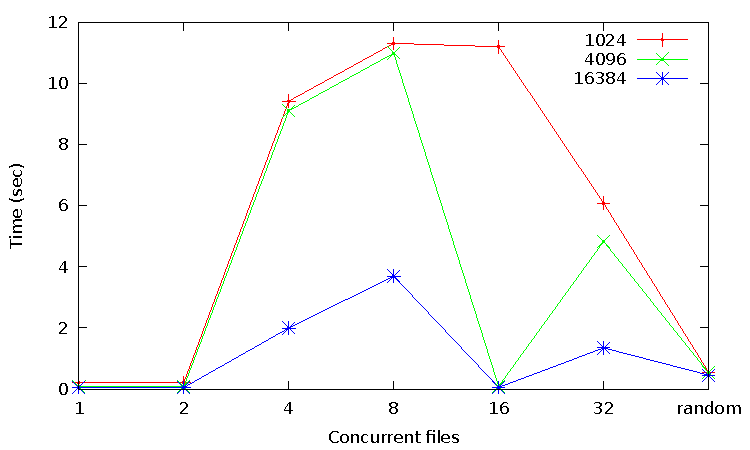
\includegraphics[width=0.5\textwidth]{res/result-sdd}
\end{figure}


\begin{table}[h!]
\caption{Lesing av fil fra USB minnepenn OS (OSX)}
\label{USB}
\centering
\begin{tabular}{|l|l|l|l|}
\hline
\multirow{2}{*}{ Antall parallelle delfiler} & \multicolumn{3}{|c|}{Blokkstørrelse} \\
 & 1024 & 4096 & 16384\\
\hline
1         &  16.234150 &   3.767864 &  3.344575 \\
2         &  20.408997 &  18.982415 &  0.663746 \\
4         &  37.190572 &  24.239117 &  4.832422 \\
8         &  37.350119 &  23.450713 &  8.085149 \\
16        &  37.177314 &  22.697717 &  7.437184 \\
32        &  36.742863 &  20.060136 &  6.026335 \\
tilfeldig &  16.653403 &   6.609872 &  8.190838 \\
\hline
\end{tabular}
\end{table}

\begin{figure}[h!]
  \caption{Plot of reading times using USB stick}
  \label{fig:usb}
  \centering
  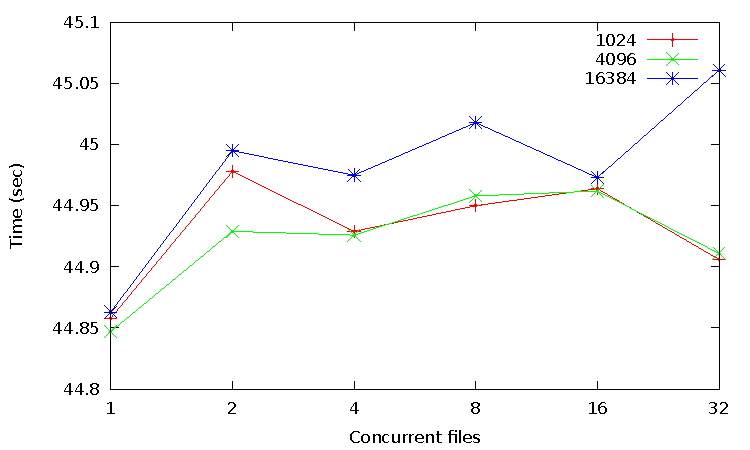
\includegraphics[width=0.5\textwidth]{res/result-usb}
\end{figure}

\begin{table}[h!]
\caption{Lesing av fil fra Harddisk (Linux)}
\label{HDD}
\centering
\begin{tabular}{|l|l|l|l|}
\hline
\multirow{2}{*}{ Antall parallelle delfiler} & \multicolumn{3}{|c|}{Blokkstørrelse} \\
 & 1024 & 4096 & 16384\\
\hline
1         &  0.164577 &  0.175946 & 0.078445 \\
2         &  0.162454 &  0.167318 & 0.080339 \\
4         &  0.165226 &  0.166446 & 0.075153 \\
8         &  0.167294 &  0.167608 & 0.074378 \\
16        &  0.167984 &  0.169632 & 0.080130 \\
32        &  0.172327 &  0.167756 & 0.076714 \\
tilfeldig &  8.910377 &  0.169295 & 4.817989 \\
\hline
\end{tabular}
\end{table}

\begin{figure}[h!]
  \caption{HDD}
  \label{fig:hdd}
  \centering
  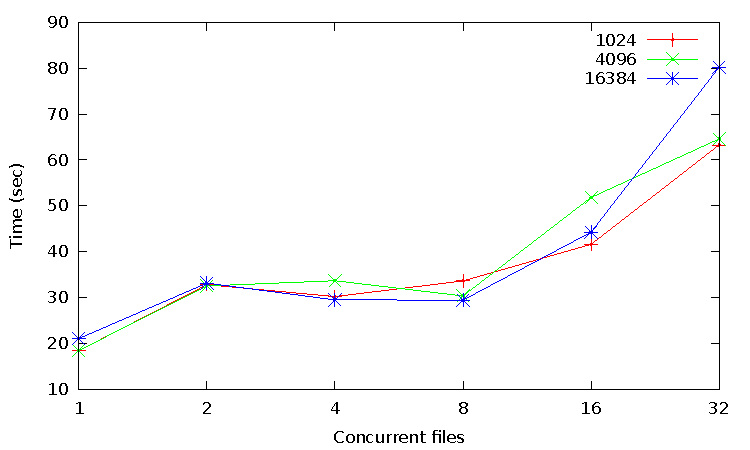
\includegraphics[width=0.5\textwidth]{res/result-hdd}
\end{figure}

Tabell \ref{SSD} og figur \ref{fig:sdd} viser kjøring ved SSD. Vi ser
en generell trend ved at økt blokkstørrelse gir lavere lesetid. Ved
økt antall parallelle åpne filer får vi noe høyere lesetid. Ved bruk
av SSD er søketiden relativt lav, slik at vi forventer at dette ikke
utgjør så mye som ved vanlig harddisk. Tabell \ref{HDD} og figur
\ref{fig:hdd} viser at dette ikke utgjør så mye som vi kunne forvente.
På grunn av praktiske hensyn er det vanskelig å sammenligne lesetid
direkte, men trendene kan likevel sammenlignes.

Lesing fra USB er, naturlig nok, veldig tregt som tabell \ref{USB} og
figur \ref{fig:usb} viser. Dette skyldes trolig at overføringen er via
USB og minnepennen var av billig modell.

Vi ser her at fra 4 til 32 parallelle filer påvirkes ikke
lesehastighet signifikant. Vi ser også her at større blokker gir
raskere lesing.



\clearpage
\section{Appendix}
\subsection{Makefile}
\lstinputlisting{../code/Makefile}

\clearpage
\subsection{benchmark.h}
\lstinputlisting{../code/benchmark.h}

\clearpage
\subsection{benchmark.cpp}
\lstinputlisting{../code/benchmark.cpp}

\clearpage
\subsection{test.cpp}
\lstinputlisting{../code/test.cpp}

\end{document}
